
\documentclass[12pt]{article} 
\usepackage{alphalph}
\usepackage[utf8]{inputenc}
\usepackage[russian,english]{babel}
\usepackage{titling}
\usepackage{amsmath}
\usepackage{graphicx}
\usepackage{enumitem}
\usepackage{amssymb}
\usepackage[super]{nth}
\usepackage{everysel}
\usepackage{ragged2e}
\usepackage{geometry}
\geometry{top=1.0in,bottom=1.0in,left=1.0in,right=1.0in}
\newcommand{\subtitle}[1]{%
  \posttitle{%
    \par\end{center}
    \begin{center}\large#1\end{center}
    \vskip0.5em}%

}
\usepackage{hyperref}
\hypersetup{
colorlinks=true,
linkcolor=blue,
filecolor=magenta,      
urlcolor=blue,
citecolor=blue,
}

\urlstyle{same}
\renewcommand*\familydefault{\ttdefault}
\EverySelectfont{%
\fontdimen2\font=0.4em% interword space
\fontdimen3\font=0.2em% interword stretch
\fontdimen4\font=0.1em% interword shrink
\fontdimen7\font=0.1em% extra space
\hyphenchar\font=`\-% to allow hyphenation
}

\begin{document}

%------------------------------------------------------------------------------------------
% Title
%------------------------------------------------------------------------------------------

\author{Michael \textsc{Brodskiy}}
\title{Final Review Packet\\European History AP}
\subtitle{Mrs Fisher}
\date{April 28, 2020}
\maketitle
\begin{center}
    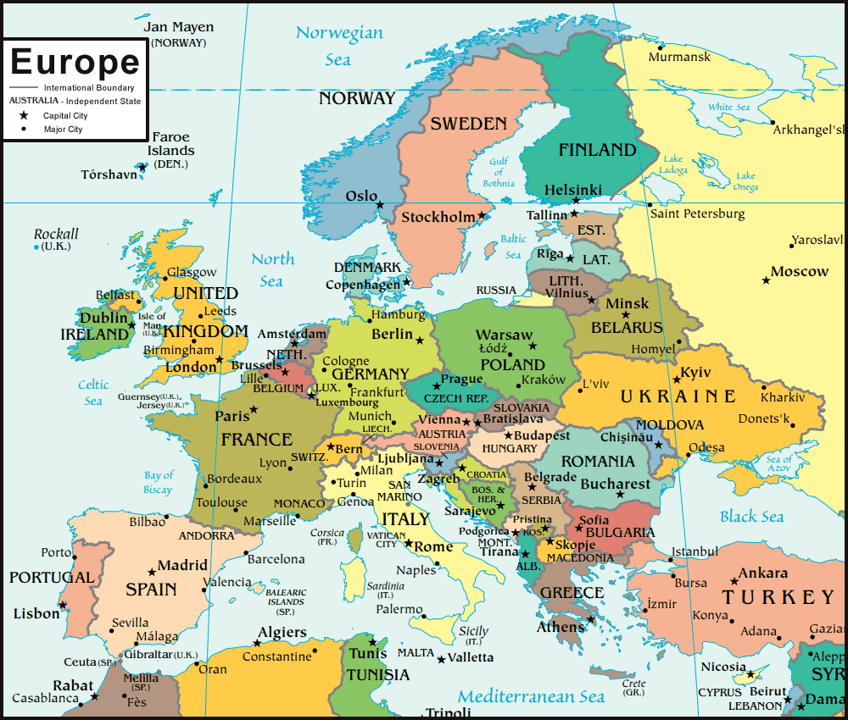
\includegraphics[width=\textwidth]{Europa.png}
\end{center}
\newpage
\tableofcontents
\newpage

%------------------------------------------------------------------------------------------
% Questions
%------------------------------------------------------------------------------------------



\begin{center}
\section{\underline{Renaissance}}
\end{center}

\begin{enumerate}[label=]
\subsection{Causes}
\item
\end{enumerate}
\vspace{-35pt}
\begin{enumerate}

\item Philosophical/Religious $-$ During the Renaissance, the term \textit{secularism} came about. This refers to something that does not relate to religion, something down-to-earth. Many artists began to paint more secular pieces, which focused on individual traits, and many were based off of classical Greek and Roman works of art. Also, many philosophers revived classical Greek and Roman thinking, and, as such, more philosophes came about.

\item Political (city states) $-$ The Italian city states did not wage war against each other for quite a bit. This created an accumulation of wealth that permitted the cities to to begin the period known as the Renaisance.

\item Economic $-$ The Renaissance began because of accumulation of wealth in Italian city states. Many Italian cities were based off of merchants and trading, and this allowed great amounts of wealth to pour in.

\item Social $-$ People became a bit more down to earth because of the new Renaissance ideals, such as: Humanism, Individualism, and Secularism.

\subsection{Terms}

\item Humanism $-$ The call back to classical Greek and Roman antiquity. This included art, architecture, and philosophy.

\item Individualism $-$ The focus on the individual as opposed to god. This stressed the importance of self value and education.

\item Secularism $-$ Down-to-earth, or not relating to religious beliefs or a god.

\subsection{People}

\item Machiavelli $-$ The author of \textit{The Prince}. He wrote this book for Cesare Borgia to demonstrate what a true Prince should act like. One of the major questions in the book is: "Which is better, to be feared or to be loved." This book offers a perspective on the royal life during the Renaissance.

\item Christine de Pisan $-$ Pisan was best remembered for defending Women in \textit{The Book of the City of Ladies}. 

\item Valla $-$ Lorenzo Valla was an early example of a humanist. He believed that pleasing the human senses was of most importance. Also, he found that a document from the 700s that granted the church rights to lots of land was a forgery.

\item Petrarch $-$ Petrarch coined the term 'Renaissance.' He began the early humanist movement. 

\item Dante $-$ Dante is the author of \textit{The Divine Comedy}. This work is considered very, if not the most important work of the Middle Ages. 

\item Boccaccio $-$ Boccaccio was an important Renaissance humanist. He wrote his book, \textit{The Decameron} in a vernacular language (meaning everyday people could read it). \textit{The Decameron} takes place near the outskirts of Florence, Italy. There are twelve people who share stories with each other. These twelve people are spending time in the outskirts of Florence to escape the raging Black Death.

\item Medici Family $-$ The Medici Family was the wealthy merchant family of Florence during the Renaissance. Because they had the greatest wealth, they were essentially the ruling family. The wealth they poured into art and the city itself spurred what is known as the Renaissance.

\item Da Vinci $-$ Da Vinci is one of the most famous artists of the Renaissance era. He was a prolific producer of art, as well as an early researcher of science. He had drawings of human anatomy, flying contraptions, and other inventions.

\item Michelangelo $-$ Michelangelo is one of the most renowned Renaissance artists. He is most famous for his work on the Sistine Chapel. To paint the ceiling, he had to spend excruciating amounts of time on his back.

\item Raphael $-$ Raphael is another Renaissance era artist. His pieces emphasized individuality and human features, as opposed to the general style of the time.

\item Alexander VI $-$ He was a corrupt pope of the Borgia Family. He encouraged his son, named Cesare, to create an Italian state ruled by their family. Alexander believed that this state was to be created by any means necessary.

\item Julius II $-$ His nickname is the "Warrior-Pope." He was involved in a lot of wara and politics. In some cases, he personally led troops to war against his enemies. He is responsible for the creation of St. Peter's Basilica.

\item Leo X $-$ Leo is responsible for the selling of indulgences. He began to sell them to fund the building of St. Peter's Basilica. Later, he would be the Pope that condemns Luther for being a heretic.

\subsection{Northern Renaissance}

\item Erasmus $-$ Desiderius Erasmus is the most famous Northern Renaissance humanist. He was of Dutch origins. He wrote \textit{The Praise of Folly}, where wrote that people should study the Bible for themselves, and that Christianity at heart, not through ceremonies was the most important.

\item More $-$ More was an early example of a Utopian Socialist. He wrote a book titled \textit{Utopia}, which comes from roots meaning 'non-existent.' In his book, he states that the government is corrupt, and that private property should not exist. He was later executed by Henry VIII for not agreeing that Henry VIII was the head of the church.

\item Durer $-$ Albrecht Durer was a painter, mostly known for three works: \textit{Devil} (1513), \textit{Melancolia I} (1514), and \textit{Rhinoceros} (1515).

\item Printing Press $-$ The printing press was made in 1454. Its main creator was Johannes Gutenberg, known for the publication of \textit{The Gutenberg Bible}. The printing press would later spur the Reformation into action, as people began to read the Bible for themselves due to the possibility of mass production permitted by the printing press.

\subsection{Compare and Contrast the Italian and Northern Renaissances}

\item Similarities $-$ Both the Italian and Northern Renaissance were inspired by classical Greek and Roman antiquity, and, therefore, were both based off of the idea of humanism.

\item Differences $-$ As opposed to the North, Italian Renaissance artists focused more on secular works. The Northern States were inspired by Christianity, and, as a result of this, Northern humanists became known as Christian humanists.

\subsection{Effects}

\item Philosophical/Religious $-$ Due to the creation of the printing press, people would begin reading the bible for themselves. This would lead to the Reformation and other religious movements.

\item Political $-$ For the duration of the Renaissance, the Italian city-states would develop a policy known as Balance of Power. This meant that if one of the states got wealthier or more powerful, the other city-states would work to even it out. The militaries of the Italian city-states, however, would prove weak following an invasion of Italy which would result in the Habsburg-Valois Wars.

\item Economic $-$ Many powerful cities, in both Italy and the North. would arise. These cities would become major trade stops for other empires. One example of such would be Amsterdam, which, for a period of time, be the center of European trade.

\item Social $-$ Following the Renaissance, books such as Castiglione's \textit{Book of the Courtier}, and Machiavelli's \textit{The Prince} would put in place social guidelines on how people in certain positions should act.

\item Education $-$ As a result of the printing press, literacy rates rose. People began to become interested in writings, such as encyclopedias, and, of course, the Bible.

\begin{center}
\section{\underline{The New Monarchs}}
\end{center}

\subsection{Causes}

\item Political $-$ The Renaissance had ushered in an era of relative peace. The New Monarchs saw this as a possibility to gain power, and, as such, they seized power.

\item Economic $-$ The New Monarchs were a direct result of the increased income during the Renaissance period. The New Monarchs needed greater revenue in order to crush political opponents and develop standing armies. As such, the period following the Renaissance was perfect for their rise.

\item Need for Permanent Standing Army $-$ The abundance of mercenaries during the Renaissance would allow for New Monarchs to establish permanent standing armies, which was something that had never been done by monarchs.

\item Taxation to Pay For Army and Bureaucracy $-$ Taxation resulted in even less money for the Peasants.

\item Classes
\begin{enumerate}[label=\arabic{*}.]
\setcounter{enumii}{36}
\item Nobles $-$ New Monarchs took power away from the nobility and placed it upon themselves. Such a move would result in a more centralized government, and thus, a more efficient bureaucracy.

\item Church $-$ As with the nobles, the New Monarchs reduced the power of the church. As such, the New Monarchs were able to create a more efficient and centralized government.

\item Middle $-$ In most of Europe, the middle class did not change very much during this time period. In Spain, however, the middle class would virtually disappear. Under the rule of Ferdinand and Isabella, the Reconquista began. This was a massive push to "Christianize" Spain. This would nearly wipe out the majority of the middle class, which consisted of the muslim Moors and Jewish people.

\end{enumerate}

\subsection{Political Situation $-$ 16\textsuperscript{th} Century}

\setcounter{enumi}{39}

\item Spain $-$ At the start of the 16\textsuperscript{th} century, Isabella had died. Ferdinand did find another queen, however they were not able to produce another heir, and, as such, Ferdinand did not have an heir from his new queen. Charles V was the most powerful ruler of Spain in the 16\textsuperscript{th} century. He fought the Habsburg-Valois war, sacked Rome in 1527, and established his main goal as the prevention of the spread of Protestantism.

\item France $-$ At the beginning of the 16\textsuperscript{th} century, France was ruled by Louis XII. He had a disastrous foreign policy, and, as such, he left an empire in trouble for his successor, Francis I. Francis I required for all bishops in churchs to be appointed by the King. He also implemented a direct tax on all property. 

\item England $-$ Before the beginning of the 16\textsuperscript{th} century, the War of the Roses was fought in England. The York family came out on top, and would then establish the Tudor dynasty. This would lead to the rise of Henry VII, the first Tudor king. Henry VII is best known for his establishment of the Star Chamber.  was the loyal right hand man of king Henry IV

\item Holy Roman Empire $-$ Maximilian I married Mary of Burgundy to obtain land in eastern France. This would spark the conflict between the House of Valois and the House of Habsburgs, and it would start the Habsburg-Valois War.

\subsection{Spain \& The Holy Roman Empire}

\item Ferdinand \& Isabella $-$ Ferdinand and Isabella ruled from 1479 to their respective deaths. Isabella died in 1504, and Ferdinand died in 1516. Together, they instigated the \textit{Reconquista}, or the reconquering of the Iberian Peninsula. They began the Catholic revival of Spain, driving out any non-Catholics. The Spanish Inquisition tortured non-Catholics into converting, fleeing Spain, or until death. This nearly destroyed the entire middle class of the Spanish Empire. 

\item Charles V $-$ Charles V was the most powerful ruler of Europe in the 16\textsuperscript{th} century. He inherited Spain and parts of most of the major contiguous European empires at the time. Leaders of the European countries were worried that Charles V would try to invade and create a world empire. 

\item Phillip II $-$ Phillip II is the son of Charles V. He is responsible for the unification of Spain with the Habsburgs. Phillip II married Mary, Queen of Scots. This showed a unification of Catholic leaders, and, as such, was a show of aggression to the English Protestants.

\subsection{England}

\item Henry VII $-$ Henry VII is the first King of the Tudor dynasty. He is best known for his establishment of the Star Chamber. His son is Henry VIII.

\item Henry VIII $-$ Henry VIII is the son of Henry VII. He married Catherine of Aragon to keep peace with Spain. Henry VIII is best known for having 6 wives. He wanted to divorce Catherine of Aragon because she only birthed daughters. The Pope, however, did not permit for Henry to divorce. As such, Henry VIII created the Anglican church through the acts of submission of clergy and supremacy. This established and declared the monarch of England the head of the Anglican church.

\item Elizabeth I $-$ Elizabeth was the daughter of Henry VIII and Anne Boleyn. She brang in an era of religious peace in England. She herself was protestant, and, as a result, she repealed any anti-protestant legislation. Her power was threatened when Mary, Queen of Scots came to England. Many people believed Mary was the true queen. Elizabeth kept Mary under house arrest, until it was revealed that there was a plan to assassinate Elizabeth. Mary was then beheaded.

\begin{center}
\section{\underline{The Age of Exploration}}
\end{center}

\subsection{Causes}

\item Political $-$ People wanted to participate in exploration to become famous. This makes up the "Glory" component of the three G's.   

\item Economic $-$ Interest in trade and spice routes fueled countries to fund explorers. Also, tales of far lands made of gold and precious metals further increased interest in exploration. This makes up the "Gold" component of the three G's.

\item Technological $-$ New inventions, such as the rudder, a piece designed to facilitate the steering of a vessel, or the caravel, a smaller ship that was effective for travel, permitted countries to engage and fund exploration.

\item Religious $-$ Also, people wanted to spread their religion through exploration. This led to the creation of missionaries that would travel on ships. This makes up the "God" component of three G's.

\subsection{People}

\item Prince Henry the Navigator $-$ Prince Henry the Navigator was Portuguese. He supported the idea of exploration so greatly, that he himself sailed on exploration voyages. He began the Age of Exploration. 

\item Columbus $-$ Christopher Columbus reached the Bahamas and parts of North and South America, thinking that it was India. As such, he called the natives "Indians." Today it is questioned whether he was a great hero or an evil man due to his mistreatment of the Native Americans.

\item Magellan $-$ Ferdinand Magellan is famous for two things relating to exploration. First, he opened the Strait of Magellan, which was extremely useful for transportation between the east and west coasts of the Americas. Second, he was the first person to circumnavigate the world. 

\item Diaz $-$ Bartholomew Diaz is one of the most famous he explorers. He is best known for his rounding of the Cape of Good Hope in 1488.

\item Da Gama $-$ Vasco da Gama is most famous for discovering a water route to India. As a direct result, the whole Italian monopoly on Asian trade was destroyed.

\item Cortes $-$ Hernando Cortes is most famous for his conquering of the Aztecs. He was searching for a city of gold, and ended up claiming Mexico for the Spanish.

\item Pizzaro $-$ While Cortes conquered in the north, Francisco Pizzaro conquered the Incas in Peru. 

\subsection{Effect on the Americas}

\item Destruction of Civilizations $-$ A direct and almost immediate result of exploration was the destruction of indigenous peoples. Although the reasons for this varied, the two most important ones are conquest and disease. People such as Cortes and Pizzaro would conquer the natives they met. Disease wiped out more natives than any other factor, as the European diseases, such as smallpox, arrived. The natives did not have any tolerance to European diseases, and, as such, contracted the diseases easily. 

\item African Slavery $-$ The market for slaves began to grow greatly, as exploration into Africa became more prevalent. Developments such as the Triangle Trade made easy access to a lucrative business for merchants. As it is to this day, people will always need cheap labor, and, as a result, the slave market grew greatly.

\subsection{Effect on Europe}

\item Intellectual $-$ With the increasing sphere of European influence in explored regions following the unilateral growth of wealth the invested European powers, primarily Spain and Portugal, gained knowledge of world geography and sailing routes to the Americas and India with respect to the European mainland.

\item Economic $-$ The economy became increasing inundated with silver and gold which inadvertently created an increase in demand of these commodities further attributing to their affluent appeal. The routes by which exchanges of the aforementioned commodities took place enabled monopolies such as the British and Dutch East India Companies to extend their transnational operations.

\item Political $-$ The formation of monopolies would further attribute to the manifestation of capitalism with relatively smaller localized governments operating analogous to the monopolies and increasing their yields of production of profitable manufacture. This model spread through most of the explored regions and would accompany European colonialism within its sphere of influence.

\subsection{Colombian Exchange} 

\item Diseases $-$ During the Colombian Exchange, many diseases were brought to and from the Americas. Most notably, smallpox was brought to America, while syphilis was brought to Europe.

\item Food $-$ Many new crops were found. These crops facilitated subsistence farming and allowed for more food availability to the average European diet. Crops brought over include, but are not limited to corn, potatoes, tomatoes, and beans.

\begin{enumerate}[label=\arabic{*}.]
\setcounter{enumii}{67}
\item Potato on Population of Northern Europe $-$ The potato was one of the most robust crops brought to Europe. It could be grown in nearly any climate, and had a good amount of calories for sustenance. As such, the population began to grow due to the surplus of food now available.
\end{enumerate}
\setcounter{enumi}{68}
\item Price Revolution (Inflation) $-$ The Price Revolution was the sharp inflation which occurred during the late period of exploration. This began in Spain and spread to other European countries.

\begin{enumerate}[label=\arabic{*}.]
\setcounter{enumii}{69}
\item Causes $-$ One reason for the Price Revolution was the growing population. The abundance of new crops caused a decrease in infant mortality rates, and, as such, an increase in population. This population required more goods, which, especially in Spain due to the nearly nonexistent middle class, could not be provided. Another reason for this inflation was the influx of precious metals such as gold and silver.

\item Effects $-$ The Price Revolution caused the Spanish economy to collapse. Other countries were worried the same would happen to them, so exploration slowed down greatly.
\end{enumerate}
\setcounter{enumi}{71}
\section{\underline{Religious Reformation}}

\subsection{Causes}

\item Religious $-$ Sale of indulgences (essentially buying forgiveness for one's sins) and other "loose morals" angered people like Luther, who believed that religion was up to the people, not the priests. Also, Luther denounced pluralism and simony, as well as Absenteeism.

\item Political $-$ One movement that fueled the Reformation was Henry VIII's switch to Anglicanism. This separated England from the pope, and would result in further spread of Protestant ideals.

\item Economic $-$ The church would take part in simony, or the selling of church offices. Also, they would sell indulgences in order to fund exploits.

\item Social $-$ Many preachers who would read the Latin version of the bible would themselves be illiterate. As such, they would preach whatever would make them more successful.

\item Northern European Renaissance Humanism $-$ The most prominent North Renaissance Humanist, Desiderius Erasmus, inspired Martin Luther. In his book, \textit{The Praise of Folly}, he criticized the church for problems such as laernign about faith through clerics. He believed that people should read the Bible for themselves.

\item Reason's for Luther's Success $-$ Luther was successful because his ideas appealed to the masses. Many people believed in salvation by faith alone, and, as such, supported Luther and his criticism of the church.

\subsection{Effects}

\item Religious $-$ The Reformation resulted in the spread of major religions that branch from Catholicism, known as Protestantism (It comes from \textit{protesting} the Catholic faith).

\item Political $-$ The biggest political effect of the Reformation was the Thirty Years' War. The Protestant-Catholic split was exacerbated by the Catholic attempts of censorship of Protestant ideas. This would directly result in the Thirty Years' War, whichw as mainly fought in the region that, modern day, is Germany.

\item Economic $-$ The Reformation supported scientific thought and acceptance of new ideas. This would lead to new inventions, which made countries richer.

\item Social $-$ People became more interested in reading the Bible for themselves, and, as such, literacy rates increased quite a bit.

\subsection{Important People}

\item Wycliffe $-$ John Wycliffe was one of the earliest church reformers. He himself was a priest. He translated the Bible to English, and was eventually pronounced a heretic.

\item Huss $-$ Jan Huss was a Czech reformer. As with all religious reformers, he was declared a heretic and was excommunicated by the church. Later, he was executed by the Holy Roman Empire.

\item Luther $-$ Luther is the most well known supporter of the Reformation. He was a German peasant who became a Catholic monk. He always disliked the church system. The final straw was the sale of indulgences, which started his revolt against the Catholic church.

\item Zwingli $-$ Ulrich Zwingli was another reformer in Switzerland. Zwinglism was almost identical to Lutheranism, except for one point: they disagreed on the Lord's Supper, better known as communion. They met at the Marburg Colloquy to discuss combining their movements, however the idea of communion kept them apart. 

\item Calvin $-$ Calvin was another Protestant reformer. His focus on religion centered around the fact of predestination $-$ that it is predetermined, at birth, whether a person will go to heaven or hell. He created the Calvinist city that is now Geneva, Switzerland. Although it began as the second most popular sect of Protestantism, behind Lutheranism, it quickly became the definition of a reformed church.

\item Henry VIII $-$ Henry VIII formed the Anglican church, and, technically, was a religious reformer in England. He broke with the church in Rome, and made the monarch the leader of the Anglican church so that he could divorce.
    
\item Edward VI $-$ Edward VI is the son of Henry VIII. He had to take the throne at nine years old. He moved the church into an extremely Protestant direction.

\item Bloody Mary $-$ Better known as Mary Tudor, she is the daughter of Henry VIII. She is known as Bloody Mary because she burned many Protestants at the stake after she restored Roman Catholicism as the religion of England.

\item Elizabeth I $-$ Elizabeth I was the daughter of Henry VIII. She was a moderate ruler. Her policy was known as \textit{Politique}, where a monarch takes the middleground between religious extremes. She allowed sermons in English, allowed priests to marry, and made the Book of Common Prayer to unite churches.

\item Mary, Queen of Scots $-$ Also known as Mary Stuart, she fled to England, but was imprisoned by Elizabeth I. This was because many people believed Mary Stuart was the rightful queen. Mary was executed after an assassination attempt on Elizabeth I was unveiled.

\item Leo X $-$ Leo X was the first to sell indulgences. He intended this system to raise moeny to rebuild St. Peter's Basilica. He condemned Luther an outlaw, and excommunicated him from the church.

\item Tetzel $-$ Tetzel promoted the sales of indulgences. He was essentially the modern day equivalent of the marketing department. He is famous for the motto about indulgences that goes: "As soon as the coin in the coffer rings, the soul from purgatory springs."

\item Frederick, Duke of Saxony $-$ The Duke of Saxony protected Martin Luther when the pope pronounced him an outlaw.

\item Charles V $-$ Charles V was the most powerful ruler of Europe in the 16\textsuperscript{th} century. He inherited Spain and parts of most of the major contiguous European empires at the time. Leaders of the European countries were worried that Charles V would try to invade and create a world empire.

\item Phillip II $-$ Phillip II is the son of Charles V. He is responsible for the unification of Spain with the Habsburgs. Phillip II married Mary, Queen of Scots. This showed a unification of Catholic leaders, and, as such, was a show of aggression to the English Protestants.

\item Ignatius Loyola $-$ Ignatius Loyola is the founder of the order of Jesuits. The Jesuits were a counter-reformationist group that would try to forcefully convert Protestants back to Catholicism.

\subsection{Terms}

\item Simony $-$ The sale of church offices.

\item Nepotism $-$ The placing of family members, rather than others, in positions of power.

\item Indulgences $-$ The sale of forgiveness of sin.

\item Babylonian Captivity $-$ A period from 1309 $-$ 1378 during which popes resided in Avignon. This was significant because it showed that the papacy could not overcome powerful rulers, as local rulers quickly seized this oppurtunity to gain control of the papacy.

\item Great Schism $-$ The Great Schism was a direct result of the Babylonian Captivity. This was a split in the church that saw the rise of three popes. Each pope had their respective support groups.

\item Protestant $-$ Any religion that stems from the Roman Catholic church and follows Reformation principles.

\item Antibaptist $-$ Also known as Anabaptists, this was a Protestant group that believed that people should not be baptized as children.

\item Salvation by Faith Alone $-$ The belief that one need simply to believe in god to make it to heaven.

\item Sole Authority of the Bible $-$ The belief that the Bible was the sole religious authority, and that it can not be overridden by anyone, even the pope.

\item Sacraments $-$ The elements that are consumed at the Eucharist, usually bread and wine. The main argument split between whether the bread and wine were only symbols or actually the body of christ.

\item Diet of Worms $-$ This was an assembly called by Charles V. Luther was ordered to attend. He was told to take back his words on the church, however Luther refused. As a result, Luther would be declared an outlaw.

\item Peasant's Revolt $-$ The German Peasants' Revolt was a direct result of Luther's preaching. These peasants interpreted Luther's preaching incorrectly. As such, Luther disapproved of this conflict, which was put down by the landowners.

\item Predestination $-$ The belief that it is decided at or before birth whether one is destined to go to heaven or not.

\item Protestant Work Ethic $-$ The belief that one's duty is to work hard and, as a result, achieve success.

\item Catholic/Counter Reformation $-$ The Counter-Reformation was a push against the ideals of the Reformation. It began at the Council of Trent. The Jesuits were formed as a machine for Catholic conversion.

\begin{enumerate}[label=\arabic{*}.]
\setcounter{enumii}{112}
\item Affirmation of Doctrines $-$ At the Council of Trent, many things were reworked. Most importantly, seven sacraments were reaffirmed.

\item Reforms of Abuses $-$ Following the Council of Trent, there were rules set in place that suppressed pluralism, simony, and indulgences.

\end{enumerate}
\setcounter{enumi}{114}
\item Council of Trent $-$ The Council of Trent was a council called into action by Pope Paul III. Its intents were to reform the church, and, hopefully, stop the spread of Protestantism. As a result of this council, the Jesuits, a religious order, would be founded.

\item Jesuits $-$ The Jesuits were a religious order that came from the "Followers of Christ." They would force Catholic conversion and exerted great political power.

\item Baroque Art $-$ This was an art and architecture style that was associated with Catholicism. It was extremely ornamental and showed life as prestigious and beautiful.

\item Church State Relations (Luther vs. Calvin) $-$ The main difference between Luther and Calvin in state relations was that Calvin believed in a theocracy. As evident by his theocracy in Geneva, he made this work. Luther, however, believed that church and state should be separated.

\item Six Articles $-$ \textit{The Six Articles of Faith} were a series of statements issued as a doctrine by Henry VIII in 1539. Henry VIII issued this to show that, although he formed the Anglican church, that he was not Protestant. The pope disagreed.

\item Peace of Augsburg (1555) $-$ This was meant as a temporary treaty with the Protestants. It declared that religion was to be decided by the many German princes in their respective areas. The Peace of Augsburg, however, did not recognize Anabaptists and Calvinists.

\section{\underline{Religious Wars}}

\subsection{Dutch Revolt (1508 $-$ 1609)}

\subsubsection{Causes}

\item Political $-$ The Protestant region in the Northern Spanish Netherlands wanted autonomy from Spain.

\item Economic $-$ One reason for this revolt was that Spain heavily taxed the Dutch workers.

\item Religious $-$ The Protestants also wanted to receive religious rights, which they wanted to achieve by breaking politically.

\subsubsection{People}

\item Philip II $-$ Phillip II is the son of Charles V. He is responsible for the unification of Spain with the Habsburgs. Phillip II married Mary, Queen of Scots. This showed a unification of Catholic leaders, and, as such, was a show of aggression to the English Protestants.

\item Duke of Alva $-$ The Duke of Alva was sent by Phillip II to put down the revolt in the Netherlands. The Duke did this, at the price of 1,500 Dutch men.

\item Elizabeth I (Spanish Armada) $-$ Phillip II would send an entire Spanish armada to attack England and eliminate Protestantism. The fleet was heavily damaged due to a storm in the English Channel, and was finished off by Francis Drake. As such, Elizabeth I led to the decline of Spain, and the rise of England as a naval power.

\subsubsection{Effects} $-$ Spain begins its decline from its golden age. England becomes the naval superpower of the world.

\subsection{French Civil War (1562 $-$ 1598)}

\subsubsection{Causes}

\item Political $-$ This was a power struggle following the death of Henry II. This involved three noble families. The War of Three Henrys was part of this civil war.

\item Economic $-$ Although this was not a directly economic conflict, the winner of this struggle would gain great riches by ascending to the throne of France. 

\item Religious $-$ This was a great religious struggle between Catholics and Huguenots, or French Calvinists.

\subsubsection{People}

\item Catherine de Medici $-$ Catherine de Medici (Part of the Medici family from the Renaissance) was the wife of Henry II. She indirectly controlled the course of the civil conflict by controlling the sons of Henry II's choices. She sided with the militant Catholics, led by the Guise family.

\item Henry IV of Navarre $-$ Henry of Navarre was one of the Henrys that participated in this struggle. He would eventually come out as the victor, and be named Henry IV. He sided with the Protestants, and would later give them rights after he would come out on top.

\item Huguenots $-$ French Calvinists.

\item St. Bartholomew's Day Massacre $-$ A mass killing of Huguenots in Paris that happened in 1572. This would elevate the religious struggles present during the French Civil Wars.

\item Edict of Nantes $-$ The treaty that was intended to end the French Civil Wars. It restored internal peace and defined the rights of the Protestants in France. 

\item Politique $-$ A policy of middle ground between Protestant and Catholic extremes.

\subsubsection{Effects} $-$ The Edict of Nantes and Peace of Augsburg would only be temporary solutions to the religious struggles. They would result in the Thirty Years' War.

\subsection{Thirty Year's War (1618 $-$ 1648)}

\subsubsection{Causes}

\item Political $-$ One reason for this conflict was the tension between the Habsburgs and French rulers.

\item Economic $-$ This war did not benefit anyone economically. Quite on the contrary, it destroyed the economies of many major European powers.

\item Religious $-$ Another reason for the war was the Catholic-Protestant tension that had existed since the Reformation.

\item Limits of Peace of Augsberg (1555) $-$ The Peace of Augsburg was only a temporary solution to the problem, as it only permitted Lutheranism, which still had limitations.

\subsubsection{The War}

\item Habsburgs vs. Most of Europe $-$ The struggle of the Thirty Years' War saw the Habsburg dynasty fight most of Europe, and even Sweden

\item Phases $-$ The phases are broken up into four parts: Bohemian (Bad), Danish (Danish Eat), Swedish (Swedish), French (Fish),

\begin{enumerate}[label=\arabic{*}.]
\setcounter{enumii}{141}

\item Bohemian (Bad) $-$ This was the first phase. It saw the Catholic victory at the Battle of White Mountain,

\item Danish (Danish Eat) $-$ This was the second phase. It saw the Catholic army, led by Wallenstein, win many battles against the Catholics.

\item Swedish (Swedish) $-$ This was the third phase. The most important event was the entrance of Gustavus Adolphus, a Swedish king. This began the turning point, where Protestants began to win.

\item French-Swedish (Fish) $-$ This was the fourth (and final) phase. At this point, France enters the war. France supported the Protestants who, thanks to this, were able to defeat the Catholics.

\end{enumerate}
\setcounter{enumi}{145}
\item Role of France $-$ Surprisingly, France entered the war on the side of the Protestants. This was a tactical move by Richelieu, the financial minister of France. This was purposefully done in order to destroy the Habsburgs, which threatened French power.

\item Defenestration of Prague $-$ Fed up with the way they were treated, Protestants began to throw Catholic officials out of windows in Bohemia. This demarcated the beginning of the Thirty Years' War.

\item Wallenstein $-$ Wallenstein was a mercenary general. During the Thirty Years' War, he fought for the Holy Roman Emperor. He defeated many Protestant armies in this war.

\item Gustavus Adolphus $-$ Entering the war in 1629, Gustavus Adolphus was, at the time, king of Sweden. He led many Protestants to victory, and was supported by Richelieu. He was killed at the battle of Luetzen in 1632.

\item Richelieu $-$ Richelieu was Louis XIII's financial minister. He pushed Louis XIII to become an absolute monarch.

\item Results (Peace of Westphalia) $-$  This was the treaty that officialy ended the Thirty Years' War. It gave rights to rulers in the Holy Roman Empire to choose their religion.

\section{\underline{Constitutionalism}}

\subsection{Tudors}

\item Henry VII $-$ Henry VII is the first King of the Tudor dynasty. He is best known for his establishment of the Star Chamber. His son is Henry VIII.

\item Henry VIII $-$ Henry VIII is the son of Henry VII. He married Catherine of Aragon to keep peace with Spain. Henry VIII is best known for having 6 wives. He wanted to divorce Catherine of Aragon because she only birthed daughters. The Pope, however, did not permit for Henry to divorce. As such, Henry VIII created the Anglican church through the acts of submission of clergy and supremacy. This established and declared the monarch of England the head of the Anglican church.

\item Edward VI $-$ Edward VI is the son of Henry VIII. He had to take the throne at nine years old. He moved the church into an extremely Protestant direction.

\item Mary I (Bloody Mary) $-$ Better known as Mary Tudor, she is the daughter of Henry VIII. She is known as Bloody Mary because she burned many Protestants at the stake after she restored Roman Catholicism as the religion of England.

\item Elizabeth I $-$ Elizabeth was the daughter of Henry VIII and Anne Boleyn. She brang in an era of religious peace in England. She herself was protestant, and, as a result, she repealed any anti-protestant legislation. Her power was threatened when Mary, Queen of Scots came to England. Many people believed Mary was the true queen. Elizabeth kept Mary under house arrest, until it was revealed that there was a plan to assassinate Elizabeth. Mary was then beheaded. She is best known for her policy of \textit{politique}.

\subsection{Stuarts}

\item James I $-$ James I was the first Tudor king. He was king of England and Ireland from 1603 $-$ 1925, and Scotland from 1567 $-$ 1625. He angered the Puritans by appointing Catholic officials. His biggest problem was that he couldn't get funding without parliament consent. 

\item Charles I $-$ Charles I was the son of James I. His and his father's need for funding resulted in the English Civil War. He was defeated in the Civil War, and was subsequently beheaded in 1649.

\item Charles II $-$ Charles II was king during the restoration period.

\item James II $-$ James II was the last Stuart king to rule England, Ireland, and Scotland. He was overthrown by William and Mary.

\item William III \& Mary II $-$ The Catholic reign of king James ened with William and Mary. They were Protestant, and, as such, required that only Protestants be allowed to hold office.

\item Anne $-$ Anne of Austria was the wife of King Louis XIII. She allowed Richelieu's successor, Cardinal Mazarin, dominate the government.

\item Cromwell $-$ Oliver Cromwell was the figure that led the Parliamentarians to victory during the English Civil War. He wanted to execute Charles I. As the leading military figure, he was placed as the ruler of England after the Civil War. Although he began as a promising ruler, he soon became dictator-like.

\subsection{Documents}

\item Magna Carta $-$ This was a royal charter that would show that the common person could fight for rights. This was made by English nobles who wanted to be treated fairly. This document stated that the king must follow the laws like any citizen. It also gave the right of \textit{Habeas Corpus}, and the right to a speedy trial.

\item Petition of Right $-$ This was a document signed by Charles I, but written by the parliament. It stated that even the monarch was subject to the laws which they pass. Charles would try to circumvent this, and would start the English Civil War as a result.

\item Habeas Corpus $-$ This gives people the right to a trial. Habeas Corpus translates as "must have the body." This protects people from being arrested arbitrarily, and requires for the government to state the reason for arrest.

\item Bill of Rights $-$ This was an English statement of fundamental rights. This looked much like the first ten amendments in the United States Constitution.

\subsection{English Civil War (1640 $-$ 1649)}

\item Causes $-$ This was caused by James and Charles I's greed for funding. They took great amounts of money from the country's wealth. Charles I would even go as far as to establish a standing army, which angered parliament. 

\item Reasons for Puritans Winning $-$ The Puritans won because Charles I was not very well organized. Charles also did not have very many supporters. The Puritans also had better leadership. As a result, the Puritans won.

\item Effects $-$ This would show that the people must guide the government. This would stand as the greatest English revolt in all of history.

\subsection{Glorious Revolution (1688)}

\item Causes $-$ James II was appointing many Catholic leaders, and thus, the Protestants felt threatened.

\item Effects $-$ This led to the formation of a constitutional monarchy in England. This was a bloodless revolt in which James II abdicated and his daughter Mary, and her husband, William of Orange, became the reigning monarchs.

\subsection{Terms}

\item Church of England $\rightarrow$ Anglican Church $-$ The Church of England, better known as the Anglican Church, was established under Henry VIII so that he would be able to divorce from his wife. This was the break of England from the Roman Catholic faith.

\item Puritans $-$  This was a group of Protestants from England that wanted to purify the Anglican church. They believed in predestination.

\item Cavaliers $-$ The cavaliers were Anglicans that believed that the king was sovereign. They defended the king and kept social order. They would mostly be found in Northwestern England. They fought the roundheads during the civil war.

\item Roundheads $-$ Named after their round haircuts, the roundheads were the gentry and merchants of London. They were Puritans that believed in private property and religious freedoms. They fought the cavaliers during the civil war.

\item New Model Army $-$ This was a trained force of Protestants that was led by Oliver Cromwell during the English Civil War.

\item Commonwealth $-$ This was the name of the Puritan republic headed by Cromwell. A constitution would be drafted, however Cromwell would not follow it, and would end up ruling as a dictator.

\item Rump Parliament $-$ The parliament that was controlled by Cromwell. It proclaimed England as a republic, and abolished the House of Lords.

\item Levellers $-$ The levellers were a group that advocated for freedom of speech, religious toleration, and a democratic republic. They wanted voting for all males over 21, and wanted male and female equality. They also supported government-funded programs for the poor and annual parliament meetings.

\item Restoration $-$ This was essentially a period that restored England to how it was before the revolution, except that Charles II headed the throne. The Parliament was more open to cooperating with the monarch, until religion became a problem.

\item Test Act $-$ The Parliament responded to Charles II with this. It stated that all military members must take an oath against transubstantiation.

\item Whigs $-$ This political party favored the Parliament over the crown.

\item Tories $-$ This was the English political party that supported royalty.

\section{\underline{Absolutism}}

\item Causes $-$ The idea of divine right, appointment to rule by god, served as the major preliminary cause of absolutist monarchism along with the accompanying beliefs that monarchs should be endowed with the ability to exercise unquestioned power derived through their relationship with god.

\subsection{French Monarchs, Ministers, and Policies}

\item Henry IV $-$ The French \textit{Good} King Henry, was a Huguenot whose acts demonstrated an unusual tolerance of accepted religious practices and textual interpretations. His support of the Edict if Nantes demarcated the end of the Wars of Religion and endowed Protestants with newfound religious liberties.

\begin{enumerate}[label=\arabic{*}.]
\setcounter{enumii}{186}

\item Edict of Nantes $-$ The treaty that was intended to end the French Civil Wars. It restored internal peace and defined the rights of the Protestants in France. %A document signed in April of 1598 effectively ending the schismatic French Wars of Religion.

\item Duke of Sully $-$ Maximilien de B\'ethune was the loyal right hand man of King Henry IV. During his tenure as a nobleman and statesman he was extremely involved in the administrative construction of a strict politically centralized governmental infrastructure. During his involvement in this new institutionalization in France he practiced efficient administrative techniques such as manipulation and coercion. 

\end{enumerate} 
\setcounter{enumi}{188}

\item Louis XIII $-$ Louis XIII was only nine years old when he took the throne. Because of his young age, his mother Marie de Medici and many wealthy nobles would control his decision making. Because he was a weak monarch, he appointed Cardinal Richelieu as hish financial minister to make up for his poor leadership.

\begin{enumerate}[label=\arabic{*}.]
\setcounter{enumii}{189}

\item Cardinal Richelieu $-$ He was the first financial minister of the crown. He exerted a great deal of influence over Louis XIII. He held the French state in high regard, and, as a result, he wanted to control all of it. This was the reason behind his push for absolutism.

\end{enumerate}
\setcounter{enumi}{190}

\item Louis XIV (The Sun King) $-$ Louis XIV was the longest ruling French king of all time. He spent lots of the state's money on somewhat frivolous purchases and costly wars. He is one of the greatest examples of an absolutist king. He is well known for his construction of the Palace of Versailles.

\begin{enumerate}[label=\arabic{*}.]
\setcounter{enumii}{191}
\item L'\'etat, C'est Moi $-$ Quoted from Louis XIV, this translates from French as, "The state, that is me." This exemplifies the absolutist power he had over the government.

\item Cardinal Mazarin $-$ This was the successor of Richelieu. He was a poor financial minister. His economic policies were not efficient, and they almost directly led to the Fronde.

\item Fronde $-$ The Fronde was an uprising that took place when Louis XIV was a child. This might explain why he was so strict on the lower classes.

\item Versailles $-$ The Palace of Versailles was a luxurious palace built during the reign of Louis XIV.

\begin{enumerate}[label=\arabic{*}.]
\setcounter{enumiii}{195}

\item Purpose/Goal $-$ Versailles was used as a "cage" for the for the nobles. It limited their power peacefully.

\item Effect $-$ Because the nobles were under control, Louis XIV had absolute power over the French state. As such, the Palace of Versailles exemplified the grandeur and power Louis XIV had.

\end{enumerate}
\setcounter{enumii}{197}

\item Bishop Bossuet (Divine Right) $-$ Bossuet was the greatest supporter of the Divine Right of Kings. He argued that the king was placed by god upon the throne, and, as such, the king did not bow down to any man or group.

\item Colbert $-$ Colbert was the financial minister for Louis XIV. He worked hard to make France economically self-sufficient. He was a great supporter of the mercantilist policy. His work brought a period of prosperity to France.

\item Mercantilism $-$ Mercantilism is the belief that a country's power was based off of its gold supply. Also, mercantilism stated that a country ought to sell more than they buy. The most important feature of mercantilism was that it required heavy government control, especially in trading industries.

\item Revocation of Edict of Nantes $-$ Louis XIV revoked the Edict of Nantes. He followed the policy of repression of Protestants, as had most of his predecessors. He argued that religious unity was paramount to a country's dignity.

\item Foreign Policy Goals $-$ Louis XIV was very aggressive in his foreign policy. He began several expensive wars. His policy was a bellicose version of "France first."

\end{enumerate}

\subsection{Wars}
\setcounter{enumi}{202}

\item Dutch Wars $-$ Louis XIV was going after revenge when he invaded the Dutch lands. He greatly wanted to suppress Dutch Calvinism. France invaded the Dutch with 100,000 troops. The Dutch had nowhere near this kind of power, and their only attempt to defend themselves was the digging of holes that would flood.

\item War of Spanish Succession $-$ After his death, Charles II did not have an heir to the throne or any instructions on what to do with the throne. As such, Phillip was chosen as the new heir, insteaed of his two sisters who were supposed to get the throne originally. This struck fear into other empires, as Phillip was related to Louis XIV, which meant France was too powerful. This would begin the War of Spanish Succession.

\item Cost $-$ Louis XIV's wars were extremely expensive, and, as such, would nearly bankrupt the French government.

\item Accomplishment $-$ Louis XIV is known for many accomplishments. First of all, his rule saw the implementation of policies that made taxation more efficient. He also improved commerce through reforms. Louis XIV also greatly improved the French military, and even appointed a Secretary of State for war. Louis XIV, however, is most remembered for being the longest ruling monarch of France.

\item Peace of Utrecht $-$ A bilateral series of peace treaties signed in the Dutch city of Utrecht, between 1713 and 1715, recognized by the belligerents in the War of the Spanish Succession.

\item Balance of Power $-$ A defining diplomatic strategy among European nations to reinforce coalitions designed to prevent dominant European nations from becoming irreversibly powerful.

\item Legacy $-$ The political and economical status of a nation or society following the previous generations foreign, domestic, and economical policy.

\item Culture \& Arts $-$ Affect by \textit{neo}-\textit{classical} Greek and Roman art, this epoch's cultural and artistic paradigms involved Romanticism and Naturalism.

\item Finances \& Taxation $-$ An inefficiently developed system in which taxation revenues where insufficiently collected from nobles and the church in a disorganized manner.

\item Economic Development $-$ Resulting from the disorganized and insufficiently developed method of taxation the French state was unable to maintain a stable financial footing.

\item Louis XV $-$ Grandson of Louis XIV and king of France from 1715 to 1774 who led France into the War of Austrian Succession and the Seven Years' War, although he was more interested with his mistresses than matters of the state he eventually took action to defend his absolutist inheritance after Parliament objection. 

\begin{enumerate}[label=\arabic{*}.]
\setcounter{enumii}{213}
 
\item Cardinal Fleury $-$ The chief minister of the French court who was essentially the last of the great clerics who loyally and effectively served the French monarchy was a realist who surrounded himself with able assistants who tried to solve France's financial problems. He died before he could successfully prevent France from intervening in the war between Austria and Prussia although his greatest failure was to prepare Louis XV to become an effective monarch.

\end{enumerate}
\setcounter{enumi}{214}

\section{\underline{Scientific Revolution \& The Enlightenment}}

\item Pre-Renaissance Science $-$ Was very limited an failed to develop a stochastic understanding of the universe. 

\begin{enumerate}[label=\arabic{*}.]
\setcounter{enumii}{215}

\item Purpose $-$ To determine the reality of the universe in terms of fathomable metrics such as distance, time, and mass.

\item Method $-$ To perform physical and thought experimentation to arrive at inductive verification of the aforementioned determinations.

\end{enumerate}
\setcounter{enumi}{217}

\item View of Universe $-$ Placed the earth at the center of the universe and assumed the planets and sun orbited the earth. This consideration wouldn't be debunked for centuries to come and was manifested in the politicization and religious influence maintained over the global scientific community.

\begin{enumerate}[label=\arabic{*}.]
\setcounter{enumii}{218}

\item Aristotle \& Ptolemy $-$ Greek born astronomers whose postulations developed the basis of accepted astronomical theory until the Scientific Revolution on the \nth{16}, \nth{17} centuries.

\item Copernicus \& Heliocentric Theory $-$ A Polish born astronomer who developed an astronomical model placing the sun at the center of the solar system. The publication of his convictions was the precipice of his social demise

\item Brahe Contribution $-$ Built an observatory and collected data from celestial sources for over two decades, although influenced greatly by Copernicus his limited informal knowledge of mathematics prevented further elaboration of the accumulated data.

\item Kepler's Contribution $-$ Applied Brahe's data to deduce that the earth's trajectory of solar orbit was elliptical. His greatest achievement was the development of 3 planetary laws of motion upon which contemporary Newtonian mechanics is based on. His worked debunked the previously considered models of Aristotle and Ptolemy.

\item Galileo's Contributions $-$ An Italian born astronomer and mathematician who was the first recorded to apply a telescope to study celestial bodies. He was able to famously demonstrate the identical descent rates among differently weighed objects.

\begin{enumerate}[label=\arabic{*}.]
\setcounter{enumiii}{223}

\item Experimentation $-$ A controlled procedure executed in accordance with conditions resembling a phenomena in order to develop determining data to arrive at an inductive verification.

\item Telescope $-$ A device constructed through the sequential refracting of light to observe distant objects by making them appear closer.

\end{enumerate}



\end{enumerate}
\setcounter{enumi}{225}

\subsection{Persecution by the Roman Catholic Church}

\item Effect on Science in Catholic Countries $-$

 
\begin{enumerate}[label=\arabic{*}.]
\setcounter{enumii}{226}

\item Newton $-$ 

\begin{enumerate}[label=\arabic{*}.]
\setcounter{enumiii}{227}

\item Law of Universal Gravitation $-$ 

\item \textit{Principia} $-$

\end{enumerate}
\setcounter{enumii}{229}

\item Bacon $-$ 

\begin{enumerate}[label=\arabic{*}.]
\setcounter{enumiii}{230}

\item Inductive Reasoning $-$ 

\item Method $-$

\item Empiricism $-$

\end{enumerate}
\setcounter{enumii}{233}

\item Descartes $-$ 

\begin{enumerate}[label=\arabic{*}.]
\setcounter{enumiii}{234}

\item Deductive Reasoning $-$ 

\item Cartesian Dualism $-$

\item "Cognito ergo su" $-$ 

\end{enumerate}

\end{enumerate}
\setcounter{enumi}{237}

\item Products of Scientific Revolution $-$

\begin{enumerate}[label=\arabic{*}.]
\setcounter{enumii}{238}

\item Intellectual $-$ 

\item Emergence of Scientific Community $-$

\item Scientific Method $-$ 

\item Belief in Reason $-$

\item Influence on Enlightenment $-$

\end{enumerate}
\setcounter{enumi}{243}
\subsection{Enlightenment}

\subsubsection{Important People}

\item Hobbes $-$ 

\begin{enumerate}[label=\arabic{*}.]
\setcounter{enumii}{244}

\item Human Nature $-$ 

\item Government $-$

\end{enumerate}
\setcounter{enumi}{246}

\item Locke $-$ 

\begin{enumerate}[label=\arabic{*}.]
\setcounter{enumii}{247}

\item Human Nature $-$ 

\item Government $-$

\end{enumerate}
\setcounter{enumi}{249}
\subsubsection{Philosophes}

\item Salons $-$ 

\item Elite vs. Masses $-$

\item Montesquieu $-$ 

\begin{enumerate}[label=\arabic{*}.]
\setcounter{enumii}{252}

\item \textit{Spirit of the Laws} $-$

\end{enumerate}
\setcounter{enumi}{253}

\item Voltaire $-$ 

\begin{enumerate}[label=\arabic{*}.]
\setcounter{enumii}{254}

\item Deism $-$ 

\item \textit{Treatise on Toleration} $-$

\item \textit{Candide} $-$ 

\item Admiration for Britain $-$ 

\item Frederick the Great $-$

\end{enumerate}
\setcounter{enumi}{259}

\item Rousseau $-$ 

\begin{enumerate}[label=\arabic{*}.]
\setcounter{enumii}{260}

\item Influence on Romantic Movement $-$ 

\item Effects of Civilization $-$

\item \textit{Social Contract} $-$

\begin{enumerate}[label=\arabic{*}.]
\setcounter{enumiii}{263}

\item General Will \& Totalitarianism $-$

\end{enumerate}
\setcounter{enumii}{264}

\item \textit{Emile}

\begin{enumerate}[label=\arabic{*}.]
\setcounter{enumiii}{265}

\item Education $-$ 

\item Treatment of Children $-$

\end{enumerate}
\end{enumerate}
\setcounter{enumi}{267}

\item Diderot $-$ 

\begin{enumerate}[label=\arabic{*}.]
\setcounter{enumii}{268}

\item \textit{Encyclop\'edie} $-$ 

\end{enumerate}
\setcounter{enumi}{269}

\item Physiocrates $-$

\begin{enumerate}[label=\arabic{*}.]
\setcounter{enumii}{270}

\item Quesnay $-$ 

\begin{enumerate}[label=\arabic{*}.]
\setcounter{enumiii}{271}

\item Laissez-faire $-$ An economic policy in which gubernatorial interests remain neutral or otherwise inexistent in economic affairs. Essentially this is doctrine of privatization under which capitalism is practiced. This is a literal translation of the French $-$ \textit{let do}.

\end{enumerate}
\setcounter{enumii}{272}

\item Adam Smith $-$ A Scottish born economist who believed that government should remain neutrally indifferent with respect to economic issues.

\begin{enumerate}[label=\arabic{*}.]
\setcounter{enumiii}{273}

\item \textit{Wealth of Nations} $-$ A publication by Adam Smith responsible for analyzing inquries into the cause of wealth and prosperity at the gubernatorial scale.

\item Capitalism $-$ An economic system in which citizens are able to accumulate profit from services and goods provided by companies operating under private ownership

\end{enumerate}

\end{enumerate}
\setcounter{enumi}{275}

\subsection{Enlightened Despotism}

\item Characteristics $-$

\begin{enumerate}[label=\arabic{*}.]
\setcounter{enumii}{276}

\item Reform of Justice and Legal Systems $-$ 

\item Improve Society \& Promote Happiness $-$

\item Religious Toleration $-$

\item Freedom of Press, etc. $-$ 

\item Economic Reform $-$ 

\item Education Reform $-$ 

\item Improve Efficiency $-$ 


\end{enumerate}
\setcounter{enumi}{283}

\item Truce Goal $-$

\subsection{Enlightened Monarchs}

\item Frederick the Great (Prussia) $-$ 

\item Peter the Great (Russia) $-$

\item Catherine the Great (Russia) $-$ 

\item Maria Theresa (Austria) $-$ 

\item Joseph II (Austria) $-$


\section{\underline{French Revolution}} 

\item \begin{tabular}{l c c c c}

Old Regime & Occupation & Taxation & Status & Problems/Gripes\\
\hline
1\textsuperscript{st} Estate & & & & \\
\hline
2\textsuperscript{nd} Estate & & & & \\
\hline
3\textsuperscript{rd} Estate & & & & \\
\hline
Bourgeoisie & & & & \\
\hline
Sans Culottes & & & & \\
\hline
Peasants & & & & \\
\hline

\end{tabular}

\subsection{Causes}

\item Finances $-$

\begin{enumerate}[label=\arabic{*}.]
\setcounter{enumii}{291}

\item Wars $-$

\item Versailles $-$

\item Interest on Debt $-$ 

\end{enumerate}
\setcounter{enumi}{294}

\item Inadequate Taxation $-$ 

\begin{enumerate}[label=\arabic{*}.]
\setcounter{enumii}{295}

\item Nobles R\'ecalcitrante $-$

\end{enumerate}
\setcounter{enumi}{296}

\item Injustice $-$

\item Enlightenment $-$ 

\item Louis XVI \& Marie Antoinette $-$

\item Parlement of Paris $-$ 

\item Estates General $-$ 

\item Cahiers de dol\'eances $-$

\item National Assembly $-$

\item Tennis Court Oath $-$ 

\subsection{1\textsuperscript{st} Phase $-$ Moderate Stage (1789 $-$ 1792)}

\item Fall of Bastille $-$ 

\item Great Fear $-$ 

\item Abolition of Feudalism $-$ 

\item Declaration of Rights of Man and Citizen $-$ 

\item Slogan $-$ 

\item Sans-Culottes Women Bring Back Royalty $-$ 

\item Financial $-$ 

\begin{enumerate}[label=\arabic{*}.]
\setcounter{enumii}{311}

\item Seizure of Church Property $-$

\item Assignats $-$ 

\end{enumerate}
\setcounter{enumi}{313}

\item Civil Constitution of Clergy $-$ 

\item Establishment of Departments $-$ 

\item Metric System $-$ 

\item Failure of Royal Family to Escape $-$ 

\item Edmund Burke $-$

\subsection{Reflections on the Revolution in France}

\item \textit{A Vindication of the Rights of Women} (Mary Wollstonecraft) $-$

\item \textit{Declaration of Rights of Women} (Olympe de Gouges) $-$

\subsection{2\textsuperscript{nd} Phase $-$ Radical Stage (1792 $-$ 1795)}

\item National Convention $-$ 

\item Jacobins $-$ 

\item Girondists $-$ 

\item Mountains $-$ 

\item Danton $-$ 

\item Marat $-$ 

\item Robespierre $-$ 

\item Declaration of Republic $-$ 

\item Execution of King and Queen $-$ 

\item Guillotine $-$ 

\item Brunswick Manifesto \& First Coalition $-$ 

\item Nationalism $-$ 

\item Levee en Masse $-$ 

\item Economic Accomodations to Sans Culottes $-$

\item Reign of Terror $-$ 

\item Committee of Public Safety $-$ 

\item Republic of Virtue $-$ 

\subsection{3\textsuperscript{rd} Phase $-$ Reactionary Stage (1795 $-$ 1799)}

\item Directory $-$ 

\item Corruption $-$ 

\subsection{Napoleonic Era (1799 $-$ 1815)}

\item Background $-$ 

\item Military Victories in Italy $-$ 

\item Invasion of Egypt $-$ 

\item Coup d'etat $-$ 

\item Consulate $-$ 

\item Emperor $-$ 

\item Concordat with the Roman Catholic Church $-$ 

\item Napoleonic Code $-$ 

\item Education Reforms $-$ 

\item Financial Reforms $-$ 


\begin{enumerate}[label=\arabic{*}.]
\setcounter{enumii}{349}

\item Bank of France $-$

\end{enumerate}
\setcounter{enumi}{350}

\item Meritocracy $-$ 

\begin{enumerate}[label=\arabic{*}.]
\setcounter{enumii}{351}

\item Legion of Honor $-$ 

\end{enumerate}
\setcounter{enumi}{352}

\item Conquest of Europe $-$ 

\item Failure of Trafalgar $-$ 

\item Foreign Policy \& Military Mistakes $-$ 

\begin{enumerate}[label=\arabic{*}.]
\setcounter{enumii}{355}

\item Continental System $-$

\item Peninsular (Spanish) War $-$

\item Invasion of Russia $-$ 

\end{enumerate}
\setcounter{enumi}{358}

\item Defeat at Battle of Nations $-$ 

\item Exile to Elba $-$ 

\item Escape from Elba \& 100 Days $-$ 

\item Battle of Waterloo \& Exile to St. Helena $-$ 

\section[\underline{Mercantilism, Agricultural Revolution, \& Industrial Revolution}]{\underline{Mercantilism and the Industrial Revolution}}

\item Mercantilism $-$ 

\subsection{Agriculture}

\item Causes $-$ 

\item Dutch \& English $-$ 
 
\begin{enumerate}[label=\arabic{*}.]
\setcounter{enumii}{365}

\item Reclamation of Land $-$

\end{enumerate}
\setcounter{enumi}{366}

\item Turnip Townshend $-$ 

\begin{enumerate}[label=\arabic{*}.]
\setcounter{enumii}{367}

\item Nitrogen-Fixing Crops $-$

\item Crop Rotation $-$

\end{enumerate}
\setcounter{enumi}{369}

\item New Farm Tools $-$ 

\begin{enumerate}[label=\arabic{*}.]
\setcounter{enumii}{370}

\item Jethro Tull $-$ Seed Drill $-$

\item Iron Plow $-$ 

\end{enumerate}
\setcounter{enumi}{372}

\item Selective Breeding of Animals $-$ 

\begin{enumerate}[label=\arabic{*}.]
\setcounter{enumii}{373}

\item Bakewell $-$

\item Protein Food $-$

\item Manure/Fertilizer $-$ 


\end{enumerate}
\setcounter{enumi}{376}

\item Enclosure Movement $-$ 

\begin{enumerate}[label=\arabic{*}.]
\setcounter{enumii}{377}

\item Effects $-$ 

\end{enumerate}
\setcounter{enumi}{378}

\subsection{Industrial Revolution}

\item Began in England in $-$ 

\item Textile Industry Inventions $-$ 

\item Steam Engine $-$ 

\item Relatively Inexpensive Iron \& Steel $-$

\item Transportation Systems $-$

\begin{enumerate}[label=\arabic{*}.]
\setcounter{enumii}{383}

\item Steam Boats/Ships $-$

\item Railroads $-$ 


\end{enumerate}
\setcounter{enumi}{385}

\item Spread of Industrialization $-$ 

\item Results $-$ 

\item Working Conditions of Proletariat $-$ 

\begin{enumerate}[label=\arabic{*}.]
\setcounter{enumii}{388}

\item Hours \& Wages $-$

\item Women $-$

\item Children $-$ 


\end{enumerate}
\setcounter{enumi}{391}

\item Sadler Committee $-$ 

\item Proletariat $-$ 

\item Change in Family Sturcture $-$ 

\item No Longer Unit of Production $-$ 

\item Just Unit of Consumption $-$ 

\item Relation of Parents to Children $-$ 

\item Urbanization $-$ 

\begin{enumerate}[label=\arabic{*}.]
\setcounter{enumii}{398}

\item Sanitation $-$

\item Crowding $-$

\item Disease $-$ 


\end{enumerate}
\setcounter{enumi}{401}

\item Luddites $-$ 

\item Increased Power of State $-$ 

\item Increased Power of Military $-$ 

\item Military Industrial Complex $-$ 

\item Reaction of Romantics $-$ 

\begin{enumerate}[label=\arabic{*}.]
\setcounter{enumii}{406}

\item Writers $-$ 

\item Composers $-$ 

\item Artists $-$  


\end{enumerate}
\setcounter{enumi}{409}

\subsection{Reaction of Economists}

\item \begin{tabular}{l c c}
\textsc{Classical School} & \textsc{Writings} & \textsc{Main Ideas} \\
\hline
Adam Smith & & \\
\hline
Malthus & & \\
\hline 
Ricardo & & \\
\hline
Benthem & & \\
\hline
John Stuart Mill & & \\
\hline
Saint Simon & & \\
\hline
Owen & & \\
\hline
Blanc & & \\
\hline
Engels & & \\
\hline
Marx & & \\
\end{tabular}

\item Basic Theories $-$

\begin{enumerate}[label=\arabic{*}.]
\setcounter{enumii}{411}

\item Economic View of History $-$

\item Class Struggle $-$

\item Inevitability of Revolution $-$ 

\item Surplus Value $-$

\item Communist Society $-$ 

\end{enumerate}
\setcounter{enumi}{416}

\section{\underline{The Congress of Vienna}}

\item Legitimacy $-$ 

\item Undue Influence of French Revolution $-$ 

\item Concert of Europe/Quadruple Alliance $-$

\item Nationalism $-$

\item Metternich in the Congress of Vienna $-$

\item \begin{tabular}{l c c c}

\hline  
Early 19\textsuperscript{th} Century: & Definition & Goals & Supporters \\
\hline
Conservative & & & \\
\hline
Reactionary & & & \\
\hline
Liberal & & & \\
\hline
Romantic & & & \\
\hline

\end{tabular}

\item German Confederation $-$

\begin{enumerate}[label=\arabic{*}.]
\setcounter{enumii}{423}

\item Carlsbad Decrees $-$

\end{enumerate}
\setcounter{enumi}{424}

\item Greek Revolution \& Independence $-$

\item Belgian Revolution \& Independence $-$

\subsection{Russia}

\item Alexander I $-$ 

\item Decembrists Revolution $-$ 

\item Nicholas I $-$ Reactionary Policies

\begin{enumerate}[label=\arabic{*}.]
\setcounter{enumii}{429}

\item Orthodoxy $-$

\item Autocracy $-$ 

\item Nationalism $-$ 

\item Secret Police $-$ 

\end{enumerate}

\setcounter{enumi}{433}

\item Alexander II $-$ 

\begin{enumerate}[label=\arabic{*}.]
\setcounter{enumii}{434}

\item Attempts at Modernization $-$

\begin{enumerate}[label=\arabic{*}.]
\setcounter{enumiii}{435}

\item Railroads $-$ 

\item Industry $-$

\end{enumerate}
\setcounter{enumii}{437}

\item Conflict Between "Westerners" \& "Slavophil" $-$

\item Assassinated $-$

\end{enumerate}
\setcounter{enumi}{439}

\item Alexander III $-$ 


\begin{enumerate}[label=\arabic{*}.]
\setcounter{enumii}{440}

\item Pogroms $-$ 

\end{enumerate}
\setcounter{enumi}{441}

\subsection{France}

\item Restoration of Louis XVIII $-$ 

\item Charles X $-$ 

\item 1830 Revolution $-$ 

\item Louis Phillipe $-$

\item Peterloo Massacre $-$ 

\item \begin{tabular}{l c c}

19\textsuperscript{th} Century Legislation & Purpose & Supporters \\
\hline
Six Acts (1819) & & \\
\hline
Repeal of Combination Acts (1824) & & \\
\hline
Great Reform Bill (1832) & & \\
\hline
Factory Act (1833) & & \\
\hline
Poor Law (1834) & & \\
\hline
Repeal of Corn Laws & & \\
\hline
Chartist Movement (1837 $-$ 1848) & & \\
\hline 
Reform Bill (1884) & & \\
\end{tabular}

\item \begin{tabular}{l c c}
\hline
19\textsuperscript{th} Century Political Parties & Goals & Supporters \\
\hline
Gladstone \& Liberals (Whigs) & & \\
\hline
Disraeli \& Conservatives (Tories) & & \\
\hline
\end{tabular}

\subsection{Irish Potato Famine}
\item British Reaction $-$ 

\item Deaths $-$ 

\item Emigration $-$

\subsection{Revolutions of 1848}

\item Nationalism $-$ 

\item Economic \& Class Struggles $-$

\item Famine $-$

\subsection{France}

\item Louis Phillipe $-$ 

\begin{enumerate}[label=\arabic{*}.]
\setcounter{enumii}{455}

\item Corruption $-$ 

\item Opposition to Expansion of Suffrage $-$ 

\item Demands for Workers' Rights $-$ 

\item Abdication $-$

\end{enumerate}
\setcounter{enumi}{459}

\item Second Republic $-$ 

\item Second Empire $-$ 

\subsection{Prussia}

\item Frederick William $-$ 

\begin{enumerate}[label=\arabic{*}.]
\setcounter{enumii}{462}

\item Freedom Press $-$ 

\item Male Suffrage $-$ 

\end{enumerate}
\setcounter{enumi}{464}

\subsection{Austrian Empire}

\item Vienna $-$ 

\item Hungary (Budapest) $-$ 

\item Czech (Prague) $-$ 

\item Northern Italy $-$ 

\subsection{German Confederation}


\item Frankfurt Assembly $-$ 

\section{\underline{Imperialism}}

\subsection{Causes}

\item Economic $-$ 

\item Military $-$ 

\item Political $-$ 

\item Religious $-$ 

\item Humanitarian $-$ 

\item Social Darwinism $-$ 

\item Sea Power $-$ 

\item Technology $-$ 

\subsection{Colonized Locations}

\item Egypt $-$

\item Africa $-$ 

\item Congo $-$ 

\item South Africa $-$ 

\subsection{Empires Involved}

\item Britain $-$ 

\item France $-$ 

\item Germany $-$ 

\item Italy $-$ 

\item Portugal $-$ 

\subsection{Britain $-$ 19\textsuperscript{th} Century}

\item Conservatives $-$ 

\begin{enumerate}[label=\arabic{*}.]
\setcounter{enumii}{487}

\item Disraeli $-$

\end{enumerate}
\setcounter{enumi}{488}

\item Liberals $-$ 

\begin{enumerate}[label=\arabic{*}.]
\setcounter{enumii}{489}

\item Gladstone $-$

\end{enumerate}
\setcounter{enumi}{490}

\item Labour Party $-$

\begin{enumerate}[label=\arabic{*}.]
\setcounter{enumii}{491}

\item Kier Hardie $-$ 

\end{enumerate}
\setcounter{enumi}{492}

\subsubsection{Reforms}

\item Vote $-$ 

\item Parliament $-$ 

\item Education $-$ 

\item Religious Toleration $-$ 

\item Food \& Drug $-$ 

\subsubsection{Ireland}

\item Home Rule Bills $-$ 

\subsection{Unification of Italy}

\item 1848 Revolution $-$ 

\begin{enumerate}[label=\arabic{*}.]
\setcounter{enumii}{499}

\item Mazzini $-$ 

\end{enumerate}
\setcounter{enumi}{500}

\item Victor Emmanuel II $-$

\item Cavour $-$ 

\item Crimean War $-$ 

\item Plombieres Agreement $-$ 

\item Austro-Sardinian War (1858) $-$ 

\item Austro-Prussian War (1866) $-$ 

\item Franco-Prussian War (1870) $-$ 

\subsection{Unification of Germany}

\item Holy Roman Empire $-$ 

\item 30 Years' War and Treaty of Westphalia $-$ 

\item Rise of Prussia $-$ 

\begin{enumerate}[label=\arabic{*}.]
\setcounter{enumii}{510}

\item Frederick William, The Great Elector $-$ 

\item Frederick I $-$ 

\item Frederick William I $-$ 

\item Frederick II $-$ 

\end{enumerate}
\setcounter{enumi}{514}

\item Napoleon $-$ 

\item Congress of Vienna $-$ 

\item Zollverein $-$ 

\item Hohenzollerns $-$ 

\item Frankfurt Assembly $-$ 

\item Kliendeutch vs. Grossdeutch $-$ 

\item Industrialization $-$ 

\item Bismarck $-$ 

\item Junkers $-$ 

\item Steps to Unification $-$ 

\begin{enumerate}[label=\arabic{*}.]
\setcounter{enumii}{524}

\item Danish War (1864) $-$ 

\item Austro-Prussian War $-$ 

\item North German Confederation (1867) $-$ 

\item Franco-Prussian War (1870 $-$ 1871) $-$ 

\end{enumerate}
\setcounter{enumi}{528}


\item Kaiser's Power $-$ 

\item Kulturkampf $-$ 

\item Social Reforms $-$ 

\item Foreign Policy $-$ 

\item Wilhelm II $-$ 

\subsection{Late 19\textsuperscript{th} Century France}

\item Napoleon III $-$ 
\begin{enumerate}[label=\arabic{*}.]
\setcounter{enumii}{534}

\item Path to Power $-$ 

\item First Phase (1851 $-$ 1860) $-$ 

\begin{enumerate}[label=\arabic{*}.]
\setcounter{enumiii}{536}

\item Domestic $-$ 

\item Foreign $-$ 

\end{enumerate}
\setcounter{enumii}{538}

\item Second Phase (1860 $-$ 1870) $-$

\begin{enumerate}[label=\arabic{*}.]
\setcounter{enumiii}{539}

\item Domestic Policy $-$ 

\item New Paris $-$ 

\begin{enumerate}[label=\arabic{*}.]
\setcounter{enumiv}{541}

\item Aesthetics $-$ 

\item Political Motivation $-$ 

\item Haussman $-$ 

\end{enumerate}
\setcounter{enumiii}{544}

\item Foreign Policy $-$

\end{enumerate}
\end{enumerate}
\setcounter{enumi}{545}


\item Franco-Prussian War $-$

\item Paris Commune (1870 $-$ 1871) $-$ 

\item Third Republic $-$


\section{\underline{Causes and Effects of War}}

\subsection{Reformation} 

\item Opponents $-$ vs.

\item Dates: to $-$

\item Location(s) $-$ 

\item Causes $-$

\item Name and Date of Treaty (If Applicable) $-$ 

\item Effects $-$ 

\subsection{30 Years' War}

\item Opponents $-$ vs.

\item Dates: to $-$

\item Location(s) $-$ 

\item Causes $-$

\item Name and Date of Treaty (If Applicable) $-$ 

\item Effects $-$

\subsection{French Civil Wars}
 
\item Opponents $-$ vs.

\item Dates: to $-$

\item Location(s) $-$ 

\item Causes $-$

\item Name and Date of Treaty (If Applicable) $-$ 

\item Effects $-$

\subsection{Dutch Rebellion}

\item Opponents $-$ vs.

\item Dates: to $-$

\item Location(s) $-$ 

\item Causes $-$

\item Name and Date of Treaty (If Applicable) $-$ 

\item Effects $-$ 

\subsection{English Civil War}

\item Opponents $-$ vs.

\item Dates: to $-$

\item Location(s) $-$ 

\item Causes $-$

\item Name and Date of Treaty (If Applicable) $-$ 

\item Effects $-$ 

\subsection{War of Spanish Succession}
 
\item Opponents $-$ vs.

\item Dates: to $-$

\item Location(s) $-$ 

\item Causes $-$

\item Name and Date of Treaty (If Applicable) $-$ 

\item Effects $-$ 

\subsection{War of Austrian Succession}

\item Opponents $-$ vs.

\item Dates: to $-$

\item Location(s) $-$ 

\item Causes $-$

\item Name and Date of Treaty (If Applicable) $-$ 

\item Effects $-$ 

\subsection{Seven Years' War}

\item Opponents $-$ vs.

\item Dates: to $-$

\item Location(s) $-$ 

\item Causes $-$

\item Name and Date of Treaty (If Applicable) $-$ 

\item Effects $-$

\subsection{Napoleonic Wars} 

\item Opponents $-$ vs.

\item Dates: to $-$

\item Location(s) $-$ 

\item Causes $-$

\item Name and Date of Treaty (If Applicable) $-$ 

\item Effects $-$ 

\item \begin{tabular}{l c c c c}

Italy & Leader(s) & Politcal/War & Economic & Intellectual/Religious \\
\hline
16\textsuperscript{th} Century & & & & \\
\hline
17\textsuperscript{th} Century & & & & \\
\hline
18\textsuperscript{th} Century & & & & \\
\hline
19\textsuperscript{th} Century & & & & \\
\hline
20\textsuperscript{th} Century & & & & \\

\end{tabular}

\item \begin{tabular}{l c c c c}

Britain & Leader(s) & Politcal/War & Economic & Intellectual/Religious \\
\hline
16\textsuperscript{th} Century & & & & \\
\hline
17\textsuperscript{th} Century & & & & \\
\hline
18\textsuperscript{th} Century & & & & \\
\hline
19\textsuperscript{th} Century & & & & \\
\hline
20\textsuperscript{th} Century & & & & \\

\end{tabular}

\item \begin{tabular}{l c c c c}

Austria & Leader(s) & Politcal/War & Economic & Intellectual/Religious \\
\hline
16\textsuperscript{th} Century & & & & \\
\hline
17\textsuperscript{th} Century & & & & \\
\hline
18\textsuperscript{th} Century & & & & \\
\hline
19\textsuperscript{th} Century & & & & \\
\hline
20\textsuperscript{th} Century & & & & \\

\end{tabular}

\item \begin{tabular}{l c c c c}

France & Leader(s) & Politcal/War & Economic & Intellectual/Religious \\
\hline
16\textsuperscript{th} Century & & & & \\
\hline
17\textsuperscript{th} Century & & & & \\
\hline
18\textsuperscript{th} Century & & & & \\
\hline
19\textsuperscript{th} Century & & & & \\
\hline
20\textsuperscript{th} Century & & & & \\

\end{tabular}

\item \begin{tabular}{l c c c c}

Russia & Leader(s) & Politcal/War & Economic & Intellectual/Religious \\
\hline
16\textsuperscript{th} Century & & & & \\
\hline
17\textsuperscript{th} Century & & & & \\
\hline
18\textsuperscript{th} Century & & & & \\
\hline
19\textsuperscript{th} Century & & & & \\
\hline
20\textsuperscript{th} Century & & & & \\

\end{tabular}

\item \begin{tabular}{l c c c c}

Portugal \& Spain & Leader(s) & Politcal/War & Economic & Intellectual/Religious \\
\hline
16\textsuperscript{th} Century & & & & \\
\hline
17\textsuperscript{th} Century & & & & \\
\hline
18\textsuperscript{th} Century & & & & \\
\hline
19\textsuperscript{th} Century & & & & \\
\hline
20\textsuperscript{th} Century & & & & \\

\end{tabular}

\item \begin{tabular}{l c c c c}

HRE/Prussia/Germany & Leader(s) & Politcal/War & Economic & Intellectual/Religious \\
\hline
16\textsuperscript{th} Century & & & & \\
\hline
17\textsuperscript{th} Century & & & & \\
\hline
18\textsuperscript{th} Century & & & & \\
\hline
19\textsuperscript{th} Century & & & & \\
\hline
20\textsuperscript{th} Century & & & & \\

\end{tabular}

\section{\underline{Events in Historical Order}}

\item 1 $-$ Renaissance

\item 2 $-$ 

\item 3 $-$ 

\item 4 $-$ 

\item 5 $-$ 

\item 6 $-$ 

\item 7 $-$ 

\item 8 $-$ 

\item 9 $-$ 

\item 10 $-$ 

\item 11 $-$ 

\item 12 $-$ 

\item 13 $-$ 

\item 14 $-$ 

\item 15 $-$

\item 16 $-$ 

\item 17 $-$ 

\item 18 $-$ 

\item 19 $-$ 

\item 20 $-$ 

\item 21 $-$ 

\item 22 $-$ 

\item 23 $-$ 

\item 24 $-$ 

\item 25 $-$ 

\item 26 $-$ 

\section{\underline{Charts}}

\item \begin{tabular}{|l|l|l|l|l|l|}

\hline
1648 & France & Spain & England & Holland & HRE \\
\hline
Political & & & & & \\
\hline
Economic & & & & & \\
\hline
Social & & & & & \\
\hline
Religion & & & & & \\
\hline


\end{tabular}

\item \begin{tabular}{|l|l|l|}

\hline
English Civil War & Causes & Effects \\
\hline
Political & & \\
\hline
Economic & & \\
\hline
Social & & \\
\hline
Religious & & \\
\hline

\end{tabular}

\item \begin{tabular}{|l|l|l|}

\hline
Term & Definition & Major People \\
\hline
Liberalism & & \\
\hline
Conservatism & & \\
\hline
Socialism & & \\
\hline
Romanticism & & \\
\hline
\end{tabular}

\item \begin{tabular}{|l|l|l|l|l|}

\hline
Revolution & Cause & Leadership & Extremes & Outcomes \\
\hline
Glorious & & & & \\
\hline
French & & & & \\
\hline
Russian & & & & \\
\hline
\end{tabular}

\item \begin{tabular}{|l|l|l|l|} 

\hline
& Vienna & Versailles & Yalta \\
\hline
Year & & & \\
\hline
People & & & \\
\hline
Why & & & \\
\hline
Positive & & & \\
results & & & \\
\hline
Negative & & & \\
results & & & \\
\hline
\end{tabular}
\section{\underline{Big Dates}}


\hspace{-25pt}\begin{tabular}{|p{.15\textwidth}|p{.25\textwidth}|p{.25\textwidth}|p{.25\textwidth}|}
\hline
Year & Event & Significance & Other \\
\hline
1454 & Printing press invented & Increased literacy & Invented by Johannes Gutenberg \\
\hline
1485$-$1603 & Length of Tudor Dynasty Rule & Creation of Court of Star Chamber & Stuart Dynasty followed Tudor rule  \\
\hline
1492 & Columbus sails the Atlantic Ocean & Beginning of Exploration Era & European Countries would compete for colonies \\
\hline
1517 & 95 Theses Posted & Demarcates the beginning of the Reformation & Written by Martin Luther  \\
\hline
1521 & Luther appears before the Diet of Worms and is excommunicated  & These events further support for Protestantism  & This encouraged Luther  \\
\hline
1534 & King Henry VIII passes the Act of Supremacy & Forms Anglican Church, with the British Monarch at its head  & Fueled the Reformation  \\
\hline
1536 & Calvin establishes Calvinism in Geneva & With the formation of an all-Calvinist state, Protestant ideals spread faster  & \\
\hline
1545$-$1563 & Length of the Council of Trent & Pushed some reforms and began the Counter-Reformation & Formed the Jesuits $-$ a religious order that sought to convert people to Catholicism  \\
\hline
1555 & Peace of Augsburg Signed & Became a temporary solution to religious problems & Would actually result in 30 Years' War \\
\hline
1588 & Spanish Armada Defeated & Showed that England became the leading naval power of Europe & \\
\hline
1598 & Edict of Nantes stops the French religious wars for a period & Gave rights to Huguenots (French Calvinists)  & Issued by Henry IV (Henry of Navarre)  \\
\hline
\end{tabular}
\newpage
\hspace{-25pt}\begin{tabular}{|p{.15\textwidth}|p{.25\textwidth}|p{.25\textwidth}|p{.25\textwidth}|}
\hline
1603$-$1714 & Length of the Stuart rule of England  & Ruled during English Civil War and the Glorious Revolution  & \\
\hline
1613$-$1917 & Length of Romanov Dynasty  & During and following the Age of Absolutism, Russia was ruled by the Romanovs  & Ended with the Russian Revolution  \\
\hline
1618$-$1648 & Length of the Thirty Years' War  & Fought over religious freedom in modern day Germany  & Protestants came from North, and Catholics from the South  \\
\hline
1643$-$1715 & Age of Louis XIV  & Known as the Sun King, he is most known for bankrupting the French treasury & Played a role in War of Spanish Succession, and caused Protestants to flee \\
\hline
1648 & End of the Thirty Years' War & Treaty of Westphalia is written & This creates relative Religious peace \\
\hline
1649 & Death of Charles I of England & Demarcates the English Civil War  & Caused Charles II to create an army to combat Cromwell \\
\hline
1688$-$1689 & Glorious Revolution in England & William and Mary of Orange rise to the throne & Creates relative peace in England \\
\hline
1689$-$1725 & Peter the Great's Rule & Russia became significantly more westernized than before  & This would open trade and other oppurtunities between Russia and the West  \\
\hline
1700s & The Enlightenment  & Became a period of free thought, in which many new philosophical ideas were created  & One of the most important periods for politics  \\
\hline
1701$-$1918 & Hohenzollern rule in Prussia & The Hohenzollerns were aggressive leaders of Prussia  & Often seen as barbarians \\
\hline
1748 & War of Austrian Succession ends  & Peace of Aix-La-Chapelle is signed  & \\
\hline
\end{tabular}
\newpage
\hspace{-25pt}\begin{tabular}{|p{.15\textwidth}|p{.25\textwidth}|p{.25\textwidth}|p{.25\textwidth}|}
\hline
1760$-$1830 & First Industrial Revolution  & A period of rapid advancement and mass production  & Most inventions today are a direct result of the Industrial Revolution, like cars, phones, computers, etc  \\
\hline
1776 & American Revolution Begins & Inspires other revolutions for freedom, such as the French and Haitian revolutions  & Also nearly bankrupted France \\
\hline
1789 & French Revolution Begins & Began a period of bloodshed that would not end until the Congress of Vienna  & Many nobles and citizens were brutally murdered  \\
\hline
1790s & A Period of French unrest  & Saw mass executions, especially during the Reign of Terror  & One of the first major uses of Secret Police to spy on 'counter-revolutionaries'  \\
\hline
1794 & The Reign of Terror  & Led by Robespierre, the Committee of Public Safety executed many innocent, but 'suspected,' counter-revolutionaries  & Caused many unnecessary deaths  \\
\hline
1804 & Napoleon becomes Emperor & Napoleon was very aggressive in his foreign policy, which is evident in the Napoleonic Wars $-$ greatly expanded France  & Left a huge legacy for the name Napoleon  \\
\hline
1814$-$1815 & Napoleon returns from exile to Elba & Begins campaign in Russia $-$ big blunder & Also called the Hundred Days \\
\hline
1815 & Congress of Vienna & Conservative European leaders met and returned Europe to pre-French Revolution state  & Kept relative peace for about 100 years  \\
\hline
\end{tabular}
\newpage
\hspace{-25pt}\begin{tabular}{|p{.15\textwidth}|p{.25\textwidth}|p{.25\textwidth}|p{.25\textwidth}|}
\hline
1830 & Revolution in France & Revolt against Charles X  & Louis Phillipe becomes King, Greeks and Belgians gain independence  \\
\hline
1832 & British Reform Bill of 1832  & This act broadened voting rights  & Proposed by the Whig party  \\
\hline
1848 & Many more revolutions shook Europe & Fueled by nationalist beliefs, revolutions broke out in France, Austria, Prussia, Italy, and many more places  & Marx and Engels also published the Communist Manifesto in 1848 \\
\hline
1852 & Napoleon III rises to the throne  & He won largely because of his name, and ruled France until 1870  & Napoleon III was the nephew of Napoleon Bonaparte  \\
\hline
1861 & Italy is Unified  & The unification of Italy would lead to the rise of Fascism  & Also, Alexandr II emancipated Russian serfs in 1861  \\
\hline
1866 & Austro-Prussian War  & Led to the decisive defeat of Austria  & \\
\hline
1870 & French first republic formed  & This was the French government from 1870 up until its loss to Germany during World War II  & Later split into occupied France and Vichy France, headed by de Gaulle.  \\
\hline
1870$-$1871 & Franco-Prussian War  & This showed that Germany had become the major power of Europe  & Although it was instigated by Bismarck, France was seen as the aggressor  \\
\hline
1871 & Unification of Germany  & United many different nations and states into one $-$ led to a build up of military  &    \\
\hline
1880$-$1914 & Imperialism  & During this period, there was a sharp rise in colonization of places with lots of natural resources, like India and Africa  & Would later be taken apart during de-Colonization, but reworked in Neocolonialism  \\
\hline
\end{tabular}
\newpage
\hspace{-25pt}\begin{tabular}{|p{.15\textwidth}|p{.25\textwidth}|p{.25\textwidth}|p{.25\textwidth}|}
\hline
1900 & Sigmund Freud publishes \textit{The Interpretation of Dreams}  & This was big because it was the first major look into psychology  & Freud was renowned for a long period, until it was discovered he was a fraud  \\
\hline
1904$-$1905 & Russian Revolution of 1905 & Resulted in a limited constitutional monarchy in Russia  &  \\
\hline
    1905 & Einstein publishes the \textit{\textsc{Special} Theory of Relativity} & His intial (\textit{special} inertial case) of the Theory of Relativity served to expand Newtonian mechanics toward relativists mechanics. This would serve as the basis for his unified field theory, which he would publish in 1916. &  The concept of $E=mc^2$ comes from this theory \\
\hline
    1914 6/28 & Archduke Franz Ferdinand is Assassinated  & Gavrilo Princip's assassination of Franz Ferdinand sparked the flame of World War I  & Gavrilo Princip was part of the \textsc{Black Hand}, a nationalist Serbian group \\
\hline
1914 7/3 & Funeral was held for Franz Ferdinand  & This Austrians would later declare war on Serbia  & \\
\hline
1917 & Russian Revolution (February)  & This led to the establishment of the Provisional Governement, with Alexandr Kerensky at the head  & The USSR would not be created until after the Octover Revolution \\
\hline
1917 & Russian Revolution (October)  & This would lead to the creation of the RSFSR, and subsequently, the formation of the Union of Soviet-Socialist Republics  & This would later cause tensions with the west because of the Communist ideals upon which the USSR was based on  \\
\hline
1918 & End of World War I & The death and bloodshed ended for about 20 years & \\
\hline
\end{tabular}
\newpage
\hspace{-25pt}\begin{tabular}{|p{.15\textwidth}|p{.25\textwidth}|p{.25\textwidth}|p{.25\textwidth}|}
\hline
1918 & Spanish Influenza Pandemic begins & The pandemic was able to spread quickly because of the poor conditions on the battlefields of Europe, and the poor understanding of biology  & The death toll is estimated to be from 20 million $-$ 50 million  \\
\hline
1919 & Treaty of Versailles is signed & Harsh punishments would lead to the rise of Hitler & Harshest clauses: Admittance of War Guilt and Reparations \\
\hline
1920 & The Age of Totalitarians Begins & Examples include: Joseph Stalin (Iossef Vissiaronovich Dzhugashvelli), Adolf Hitler, and Mussolini  & \\
\hline
1921$-$1927 & Lenin's New Economic Policy  & The NEP (New Economic Policy) was a form of socialism with some capitalist policies that allowed citizens to sell their grain surpluses  & The NEP failed greatly  \\
\hline
1923 & End of Weimar hyper-inflation  & The period from 1921$-$1923 saw the hyper-inflation of the German Mark  & \\
\hline
1928 & The Kellogg-Briand Pact Signed  & This treaty proclaimed that war was not to be used as an instrument of foreign policy  & This treaty failed miserably at preventing the Second World War  \\
\hline
1929 & The Great Depression Begins  & Following Black Tuesday, all of the world's capitalist economies would collapse   & Caused famines and shortages across the globe \\
\hline
\end{tabular}
\newpage
\hspace{-25pt}\begin{tabular}{|p{.15\textwidth}|p{.25\textwidth}|p{.25\textwidth}|p{.25\textwidth}|}
\hline
1930$-$1935 & France's Maginot Line  & This was a series of concrete barriers and bunkers that were meant to prevent a German attack on France  & This failed miserably, as Germany would flank France through Belgium  \\
\hline
1933 & Hitler Becomes Chancellor of Germany & This would lead to World War II and the Holocaust  & Hitler succeeded greatly thanks to the policy of appeasement used by the West  \\
\hline
1936 & Rome-Berlin Axis  & This treaty was signed in order to unite Germany and Italy  & Germany and Italy became close through the Spanish Civil War  \\
\hline
1936 & Remilitarization of the Rhineland  & Hitler sent a squad of armed forces to the Rhineland, clearly in violation of the Locarno Pact  & Hitler got away with this thanks to appeasement  \\
\hline
1938 & Kristallnacht & Orchestrated by Hitler, this night saw raiding of Jewish shops and murder of Jewish people in Germany & Translates to "Night of Broken Glass" \\
\hline
1939 & Molotov-Ribbentrop Pact Signed  & Germant signed this non-aggression pact with the Soviet Union in order to prevent, at least for the beginning, a two-front war  & Stalin agreed to this because he wanted to split Poland in order to create a buffer between the Soviet Union and Germany  \\
\hline
1939 & Invasion of Poland demarcates German aggression & This marked the beginning of World War II & Bloodshed begins \\
\hline 
1940 & Invasion of France & France surrenders to Germany after roughly one month of battling & Germany's Blitzkrieg proves extremely successful \\
\hline
1941 & Invasion of the Soviet Union & June 22nd, 1941 marks the day Operation Barbarossa (Hitler's invasion plan) begins & The Great Patriotic War would last roughly 3 years \\
\hline
\end{tabular}
\newpage
\hspace{-25pt}\begin{tabular}{|p{.15\textwidth}|p{.25\textwidth}|p{.25\textwidth}|p{.25\textwidth}|}
\hline
1944 & Invasion of Normandy & The storming back of Europe involved the United States, Britain, and Canada & Germans were pushed closere to Berlin  \\
\hline
1945 & V-E Day  & Beginning with the Soviet entrance into Berlin, this marked the end of the Second World War  & Tensions between the West and the Soviet Union rose quickly following the fall of Germany  \\
\hline
1945 & U.S. Drops Atomic bomb on Hiroshima  & First aggressive use of the a-bomb & Japanese still do not surrender \\
\hline
1945 & U.S. Drops Atomic bomb on Nagasaki  & Second aggressive use of the a-bomb & Japanese surrender  \\
\hline
1945 & V-J Day  & Japan surrenders to the United States  & Japanese had to sign their surrender on an American ship  \\
\hline
1945 & Yalta/Potsdam Conferences  & Discuss plans for Germany post-war  & Do not discuss Eastern Europe $-$ this caused a rise in tension during the cold war  \\
\hline
1946 & Churchill gives his most famous speech  & Churchill comes up with the quote that an "Iron Curtain" has covered Europe  & This quote is often used to refer to the Soviet Union's hold over Europe  \\
\hline
1947 & The Central Intelligence Agency was founded  & An extension of U.S. Foreign Policy & This was the first civilian-based intelligence analyzing and gathering agency  \\
\hline
1948 & The Berlin Airlift takes place  & After a Soviet blockade of West Berlin, the United States and Britain decided to carry out "Operation Vittles"  & This lasted until 1949  \\
\hline
1949 & NATO(North Atlantic Treaty Organization) is founded & It was created as an alliance against possible Soviet aggression & Soviet Union would respond with the WTO(Warsaw Treaty Organization) \\
\hline
1953 & Stalin dies  & Caused a scramble for the position of Leader of the Soviet Union  & Khrushchev (after a short period of Malenkov) becomes leader \\
\hline
\end{tabular}
\newpage
\hspace{-25pt}\begin{tabular}{|p{.15\textwidth}|p{.25\textwidth}|p{.25\textwidth}|p{.25\textwidth}|}
\hline
1958 & The Fifth Republic in France Begins  & Charles de Gaulle becomes president of the Fifth Republic of France  & \\
\hline
1961 & Berlin Wall Built  & The Berlin wall is a perfect example of the "Iron Curtain" that surrounded Europe during the Cold War  & People were not allowed to cross from East Germany to West  \\
\hline
1968 & Czechoslovakian Uprising Occurs  & The Prague Spring began with the election of Alexander Dub\u cek, but was later crushed by the Soviets  & The Czechoslovakian Uprising is also called the Prague Spring  \\
\hline
1979 & Soviet Invasion of Afghanistan begins  & Although this was meant to be a quick invasion, it lasted significantly longer due to the death of Leonid Brezhnev  & The invasion was also lengthened due to the Central Intelligence Agency's subversive actions and support of the Afghan counter-revolutionaries  \\
\hline
1980 & Ronald Reagan elected into office  & Reagan strongly opposed Soviet rule, and, as such, had an iron foreign policy when dealing with the Soviets  & Reagan referred to the Soviet Union as "The Evil Empire"  \\
\hline
1985 & Gorbachev becomes the leader of the Soviet Union  & He implemented his policies, known as Glasnost and Perestroika  & His rule led to a period of relative relaxation, known as D\'etente  \\
\hline
1988 & Demonstrations and subsequent freedom in Czechoslovakia  & Protests in Czechoslovakia and the weakening of the Soviet system led to the freeing of Czechoslovakia from communist rule  & \\
\hline
\end{tabular}
\newpage
\hspace{-25pt}\begin{tabular}{|p{.15\textwidth}|p{.25\textwidth}|p{.25\textwidth}|p{.25\textwidth}|}
\hline
1990 & East and West Germany Unify  & This showed that the era of Soviet rule was over, and that the Cold War was coming to a stop  &   \\
\hline
1991 & Yugoslavia begins to disintegrate & This would be the beginning of the nationalist schisms and conflicts in the Balkans  & Most notable is the conflict between Serbia and Albania  \\
\hline
1991 & Soviet Union collapses & This was the end of the Cold War  & Marked the end of Communist vs. Capitalist, but not East vs. West  \\
\hline
\end{tabular}


\section{\underline{People}}

\begin{tabular}{|l|l|l|l|}
\hline
Conflicting & Issues of & Time \& & Impact \\
Personalities & Conflict & Place & \\
\hline
Wilson vs. & & & \\
Clemenceau & & & \\
\hline
Bismarck vs. & & & \\
Napoleon & & & \\
\hline
Lenin vs. & & & \\
Kerensky  & & & \\
\hline
Galileo vs. & & & \\
Urban & & & \\
\hline
Metternich & & & \\
Italy & & & \\
\hline
Luther vs. & & & \\
Charles V & & & \\
\hline
Cromwell vs. & & & \\
Charles & & & \\
\hline
Truman vs. & & & \\
Stalin & & & \\
\hline
Phillip II vs. & & & \\
Elizabeth I & & & \\
\hline
Hitler vs. & & & \\
Chamberlain & & & \\
\hline


\end{tabular}

\begin{tabular}{|l|l|l|l|l|l|}

\hline
 & 16\textsuperscript{th} & 17\textsuperscript{th} & 18\textsuperscript{th} & 19\textsuperscript{th} & 20\textsuperscript{th} \\
\hline
Most & & & & & \\
influential & & & & & \\
politician & & & & & \\
\hline
Greatest & & & & & \\
intellectual & & & & & \\
& & & & & \\
\hline
Greatest & & & & & \\
artist & & & & & \\
& & & & & \\
\hline
Famous & & & & & \\
economist & & & & & \\
    & & & & & \\
\hline
Bad Guy & & & & & \\
    & & & & & \\
    & & & & & \\
\hline
Good Guy & & & & & \\
    & & & & & \\
    & & & & & \\
\hline

\end{tabular}

\begin{tabular}{|l|l|l|l|l|l|}

\hline
Master & Political & Economic & Religious & Social & Intellectual\\
PERSIA & & & & & \\
\hline
1450 & & & & & \\
\hline
1650 & & & & & \\
\hline
1789 & & & & & \\
\hline
1815 & & & & & \\
\hline
1848 & & & & & \\
\hline
1870 & & & & & \\
\hline
1914 & & & & & \\
\hline
1918 & & & & & \\
\hline
1939 & & & & & \\
\hline
1945 & & & & & \\
\hline
1964 & & & & & \\
\hline



\end{tabular}

\end{enumerate}



\end{document}












